\chapter{Resultados}
\label{ch:results}
En esta sección se presentan y analizan los resultados obtenidos a partir de la visualización teórica del comportamiento de diversos algoritmos de multiplicación de enteros. Donde los gráficos generados permiten observar tendencias esperadas en tiempo de ejecución, uso de memoria y eficiencia relativa. 

Se incluyen representaciones gráficas como:

\begin{itemize}
    \item Gráfico de tiempo vs tamaño de entrada
    \item Gráfico de barras comparativo
    \item Diagrama de caja (boxplot) para variabilidad
\end{itemize}

\section{Análisis y visualización}
En esta sección se presentan los resultados obtenidos a partir de la implementación y simulación de distintos algoritmos de multiplicación de enteros.

\clearpage

\subsubsection{Gráfico de barras}

\begin{figure}[!ht]
    \centering
    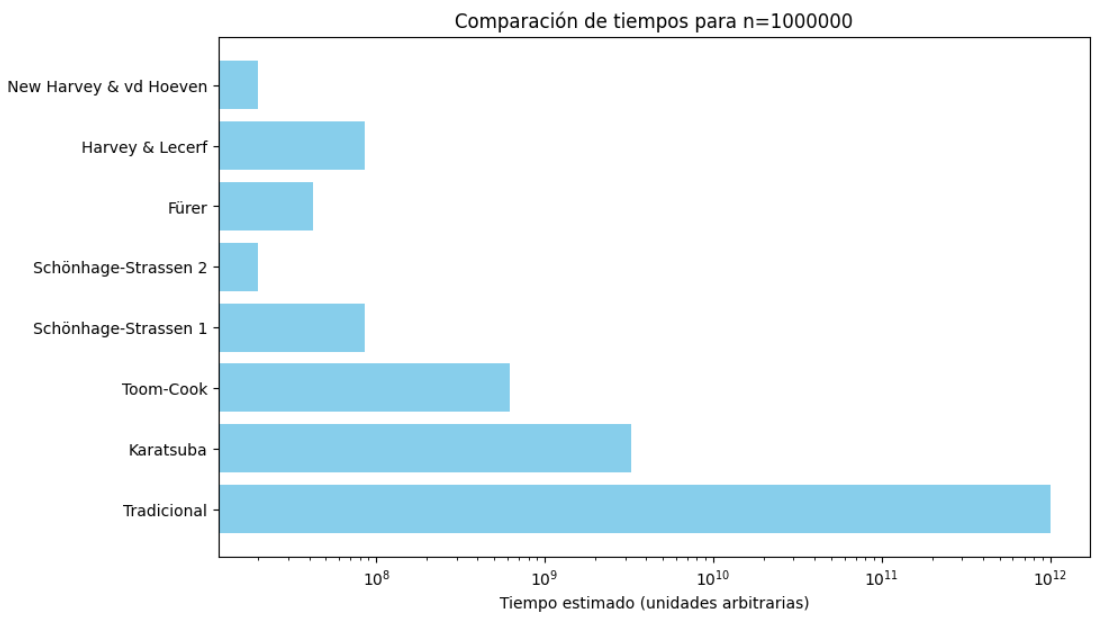
\includegraphics[scale=0.7]{figures/graficobarras.png}
    \caption{Gráfico de barras}
    \label{fig:chart_a}
\end{figure}


\paragraph{Análisis} 
El gráfico de barras permite comparar directamente el tiempo teórico que cada algoritmo requeriría para multiplicar dos enteros de un tamaño fijo. Se observa que los algoritmos clásicos, como la multiplicación tradicional (\(O(n^2)\)), presentan tiempos considerablemente mayores frente a métodos más avanzados como Karatsuba o Toom-Cook y estos a su vez presentan tiempos superiores a los presentes en New Harvey-van der Hoeven algorithm y Schönhage-Strassen second algorithm.

\clearpage

\subsubsection{Gráfico de tiempo vs tamaño de entrada}

\begin{figure}[!ht]
    \centering
    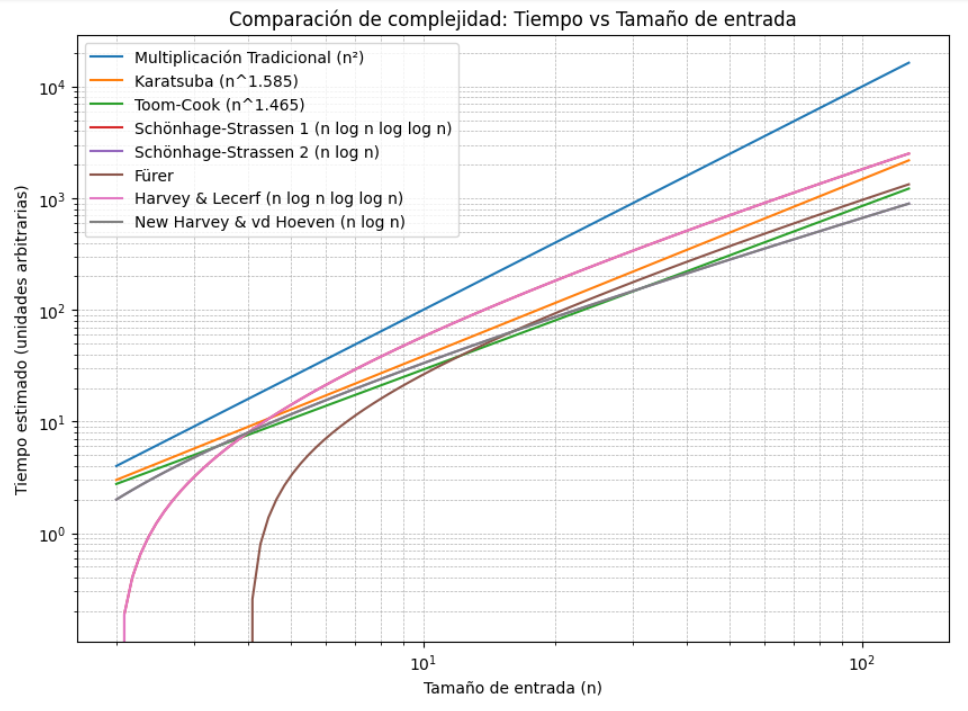
\includegraphics[scale=0.7]{figures/graficotvst.png}
    \caption{Gráfico de tiempo vs tamaño de entrada}
    \label{fig:chart_a}
\end{figure}

\paragraph{Análisis}
El gráfico de tiempo vs tamaño de entrada permite comparar directamente el tiempo teórico que cada algoritmo requeriría. Se observa que los algoritmos clásicos, como la multiplicación tradicional (\(O(n^2)\)), presentan un crecimiento prácticamente cuadrático. En contraste, los métodos más avanzados muestran un crecimiento más lento en el eje vertical (tiempo), lo que genera una curvatura visible que se acentúa a medida que mejora la complejidad algorítmica. Esta curvatura refleja cómo los algoritmos más eficientes escalan mejor con tamaños de entrada crecientes, ofreciendo un rendimiento teóricamente superior.

\clearpage

\subsubsection{Gráfico de caja}

\begin{figure}[!ht]
    \centering
    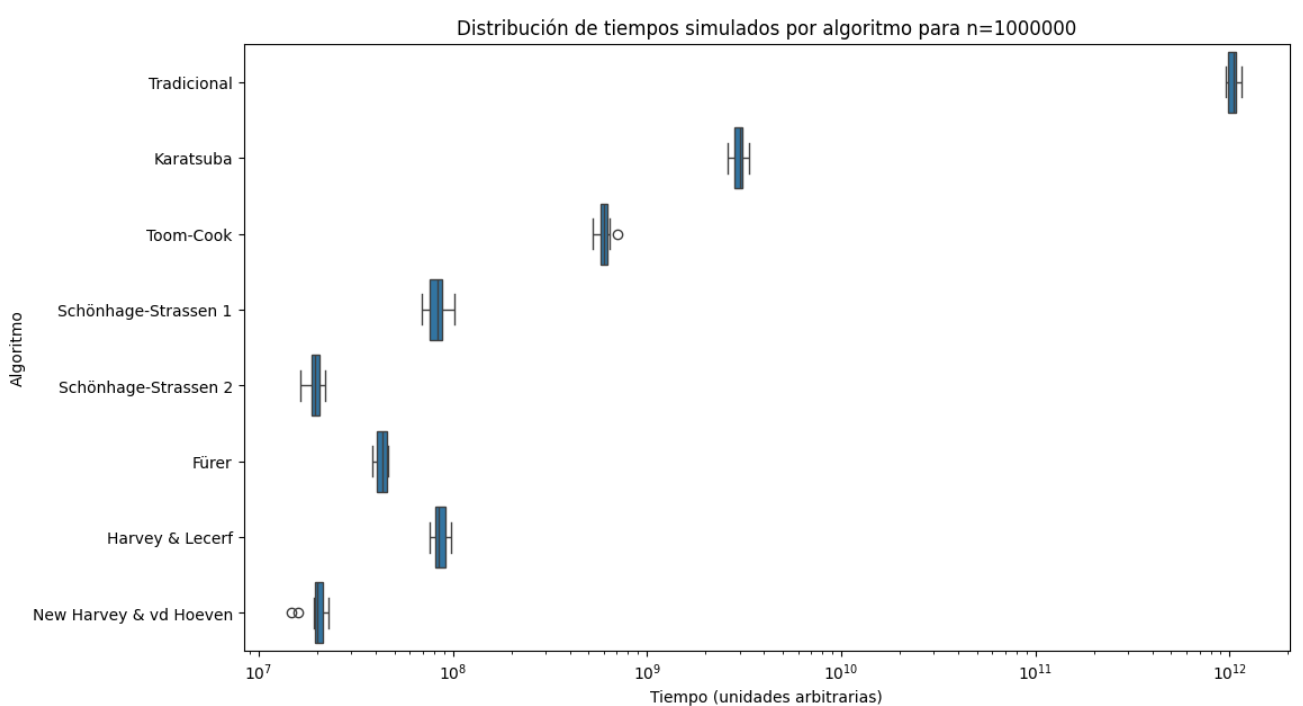
\includegraphics[scale=0.6]{figures/graficocajas.png}
    \caption{Gráfico de caja}
    \label{fig:chart_a}
\end{figure}

\paragraph{Análisis}
El gráfico de caja permite visualizar la variabilidad del tiempo teórico entre algoritmos en diferentes tamaños de entrada. Cada caja representa la distribución de tiempos para un algoritmo específico, permitiendo observar la mediana, los cuartiles y posibles valores atípicos. Se evidencia que los algoritmos con mayor complejidad, como la multiplicación tradicional, tienden a tener una dispersión más amplia a medida que el tamaño de entrada crece. En cambio, los algoritmos más eficientes presentan cajas más compactas, lo que indica una mayor estabilidad y menor variación teórica del tiempo de ejecución. Esta visualización resulta útil para comparar no solo el rendimiento promedio, sino también la consistencia de cada enfoque.
\clearpage

\section{Comparación general}

\paragraph{Complejidad asintótica} 
Los algoritmos muestran una evolución clara desde la multiplicación tradicional con complejidad cuadrática \( O(n^2) \), hasta algoritmos más avanzados como Karatsuba \( O(n^{1.585}) \), Toom-Cook \( O(n^{1.465}) \), y finalmente el algoritmo de Harvey–van der Hoeven con complejidad óptima \( O(n \log n) \). La tendencia decreciente dentro de la complejidad representa para nosotros avances significativos en eficiencia teórica.

\paragraph{Visualización de rendimiento} 
Los gráficos generados evidencian la diferencia en el crecimiento del tiempo teórico a medida que se incrementa el tamaño de entrada. Mientras que los algoritmos clásicos presentan curvas que crecen rápidamente, los algoritmos modernos muestran un crecimiento mucho más moderado.

\paragraph{Aplicabilidad práctica} 
Si bien algunos algoritmos modernos ofrecen mejor rendimiento teórico, su implementación puede ser más compleja y especializada. En la práctica, algoritmos como Karatsuba o Toom-Cook ofrecen una buena relación entre eficiencia y facilidad de implementación, siendo útiles para tamaños de entrada medianos.
